\documentclass{beamer}

% \usepackage{beamerthemesplit} // Activate for custom appearance
\usetheme{Malmoe}
\setbeamertemplate{footline}[page number]{}
\usepackage{graphicx,subfig,float, movie15, animate, xmpmulti, multicol, dsfont, hyperref}
\usepackage{multirow}
\usepackage{rotating}

\title{Digits Recognizer}
\author[Group 2]{Group 2\\ {\small G.X. Liu, D.W. Chen and K.I. Chung}}

\date{June 21, 2017}

\begin{document}
%%%%%%%%%%%%%%%%%%%%%%%%%%%%%%%%%%%%%%%%%%%%
\frame{\titlepage}
%%%%%%%%%%%%%%%%%%%%%%%%%%%%%%%%%%%%%%%%%%%%
\section[Outline]{}
\frame{
\begin{columns}
\begin{column}{.6\textwidth}
\tableofcontents
\end{column}
\begin{column}{.4\textwidth}
\url{https://goo.gl/Ac1aXg}
\centering

\includegraphics[width = \textwidth]{QR.png}
\end{column}
\end{columns}
}
%%%%%%%%%%%%%%%%%%%%%%%%%%%%%%%%%%%%%%%%%%%%
\section{Introduction}
\subsection{Data Resource}
\frame{
\frametitle{The Handwritten Digits}
They are originally from the MNIST database.
\begin{itemize}
\item 60000 training data
\item 10000 test data
\end{itemize}
Now, it is a competition on the Kaggle.
\begin{itemize}
\item 42000 training data
\item 28000 test data
\end{itemize}
}
%%%%%%%%%%%%%%%%%%%%%%%%%%%%%%%%%%%%%%%%%%%%
\subsection{Information}
\frame{
\frametitle{Information}
\begin{itemize}
\item Images contain $28 \times 28$ pixels.
\item There are 784 independent variables.
\item The response labels the real values of images.
\end{itemize}

\begin{table}[htp]
\caption{Frequency of Digits}
\begin{center}
\begin{tabular}{c|ccccc}
digit	&	0 	&	1    	&	2    	&	3    	&	4    	\\
freq. 	&	4132	&	4684	&	4177	&	4351	&	4072 \\ \hline 
digit	&	5    	&	6    	&	7    	&	8    	&	9 	 \\
freq. 	&	3795	&	4137	&	4401	&	4063	&	4188	 \\
\end{tabular}
\end{center}
\label{default}
\end{table}%
}

%%%%%%%%%%%%%%%%%%%%%%%%%%%%%%%%%%%%%%%%%%%%
\frame{
\frametitle{Representation}
\qquad The function, $f$ transfers an observation with 784 variables into an $28 \times 28$ image matrix.
\begin{equation*}
f: \mathds{R}^{784} \rightarrow M_{28 \times 28}
\end{equation*}
\begin{equation*}
M = 
	\begin{bmatrix}
		\text{pixel}_{000}	&	\text{pixel}_{001}	&	\cdots	&	\text{pixel}_{027} \\
		\text{pixel}_{028}	&	\text{pixel}_{029}	&	\cdots	&	\text{pixel}_{055} \\
		\vdots			&	\vdots			&	\ddots	&	\vdots		   \\
		\text{pixel}_{756}	&	\text{pixel}_{757}	&	\cdots	&	\text{pixel}_{783} 
	\end{bmatrix}_{28 \times 28}
\end{equation*}

}

%%%%%%%%%%%%%%%%%%%%%%%%%%%%%%%%%%%%%%%%%%%%
\subsection{Image Examples}
\frame{
\frametitle{Images from the Training Data}
\begin{figure}[htbp]
\begin{center}
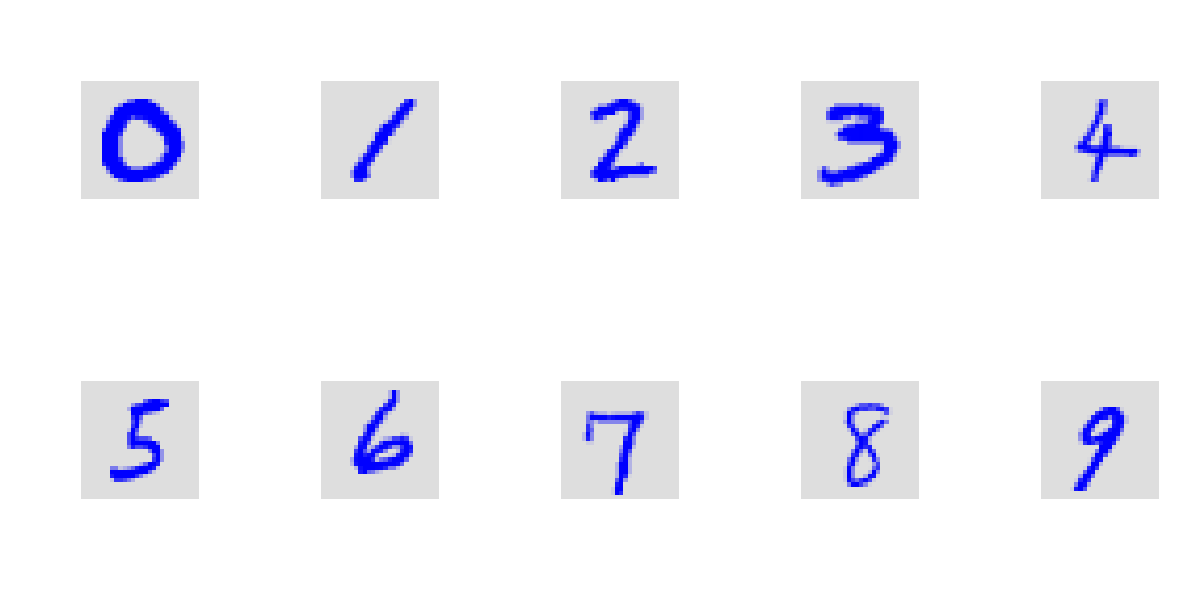
\includegraphics[width = 4.5 in]{figure/fig_ex_trn.pdf}
\end{center}
\end{figure}
}
%%%%%%%%%%%%%%%%%%%%%%%%%%%%%%%%%%%%%%%%%%%%
\frame{
\frametitle{Images from the Test Data}
\begin{figure}[htbp]
\begin{center}
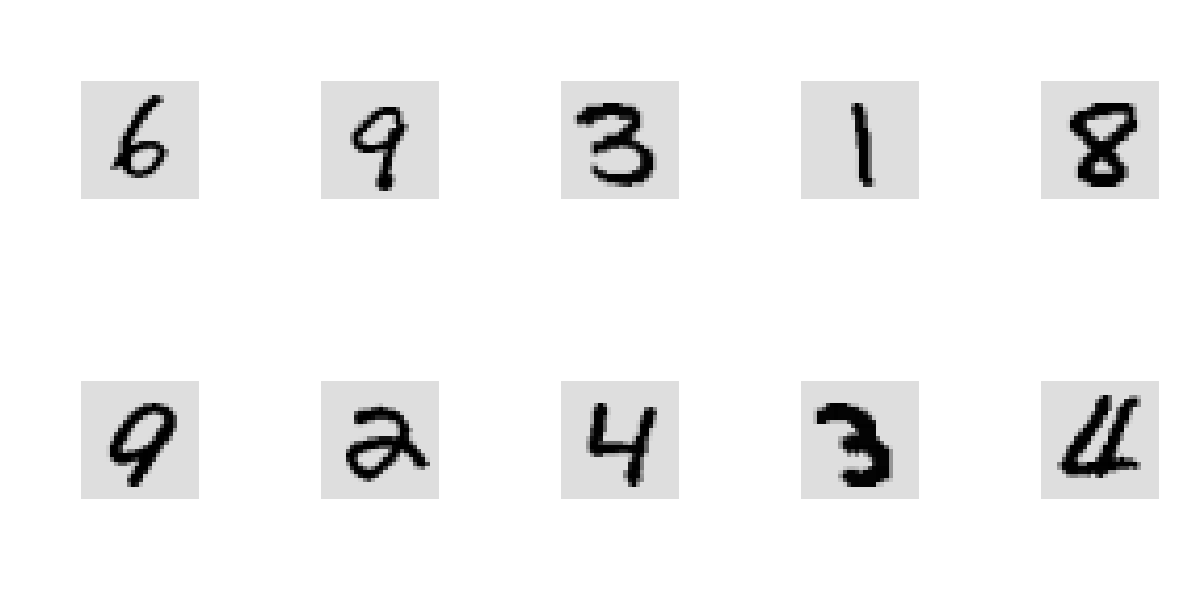
\includegraphics[width = 4.5 in]{figure/fig_ex_tst.pdf}
\end{center}
\end{figure}
}


%%%%%%%%%%%%%%%%%%%%%%%%%%%%%%%%%%%%%%%%%%%%
\frame{
\frametitle{Some Naked-eyed Unrecognizable Images}
\begin{figure}[htbp]
\begin{center}

\includegraphics[width = 4.5 in]{figure/fig_weird.pdf}
\end{center}
\end{figure}
}


%%%%%%%%%%%%%%%%%%%%%%%%%%%%%%%%%%%%%%%%%%%%
\section{Summary Statistics}
\subsection{Means}
\frame{
\frametitle{The Mean Images of the Different Digits}
\begin{figure}[htbp]
\begin{center}
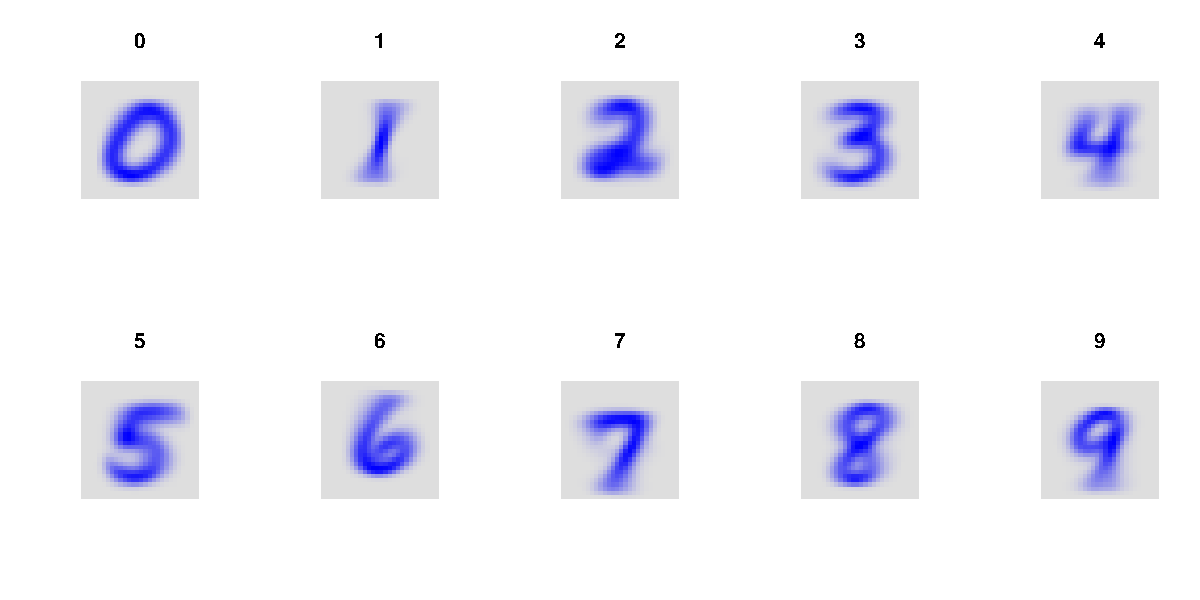
\includegraphics[width = 4.5 in]{figure/fig_mean_digit.pdf}
\end{center}
\end{figure}
}

%%%%%%%%%%%%%%%%%%%%%%%%%%%%%%%%%%%%%%%%%%%%
\frame{
\frametitle{The Mean Curves of the Different Digits}
\begin{figure}[htbp]
\begin{center}
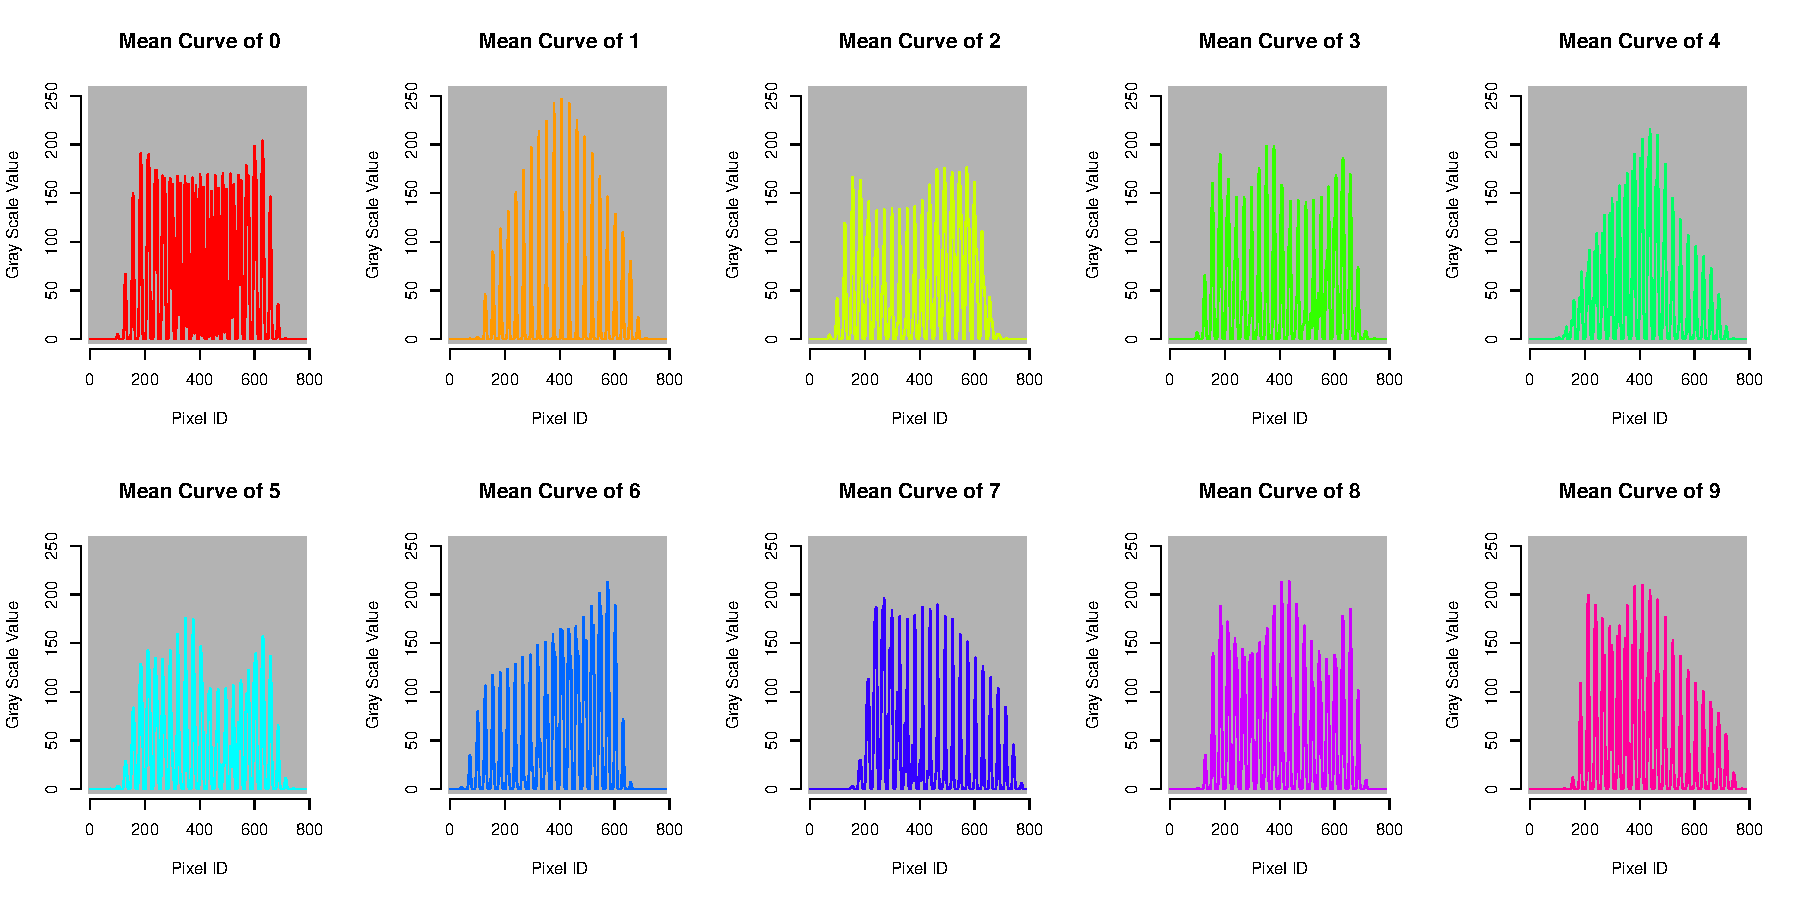
\includegraphics[width = 4.5 in]{figure/fig_mean_curve.pdf}
\end{center}
\end{figure}
}

%%%%%%%%%%%%%%%%%%%%%%%%%%%%%%%%%%%%%%%%%%%%
\frame{
\frametitle{The 20\% Trimmed Mean Images of the Different Digits}
\begin{figure}[htbp]
\begin{center}
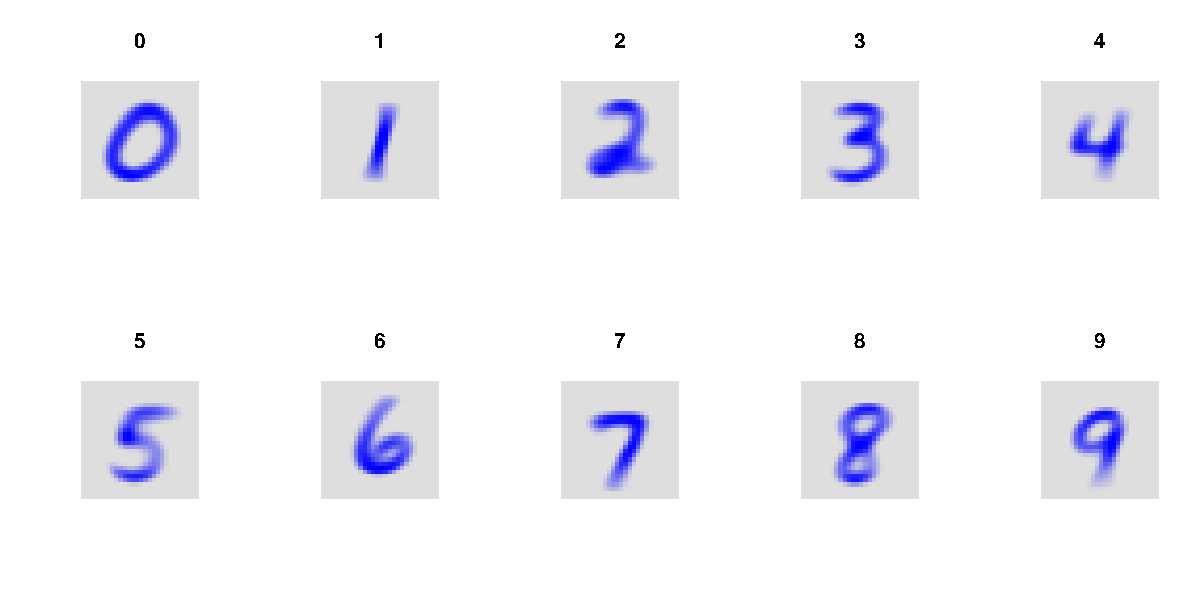
\includegraphics[width = 4.5 in]{figure/fig_mean_digit_trim.pdf}
\end{center}
\end{figure}
}

%%%%%%%%%%%%%%%%%%%%%%%%%%%%%%%%%%%%%%%%%%%%
\frame{
\frametitle{The 20\% Trimmed Mean Curves of the Different Digits}
\begin{figure}[htbp]
\begin{center}
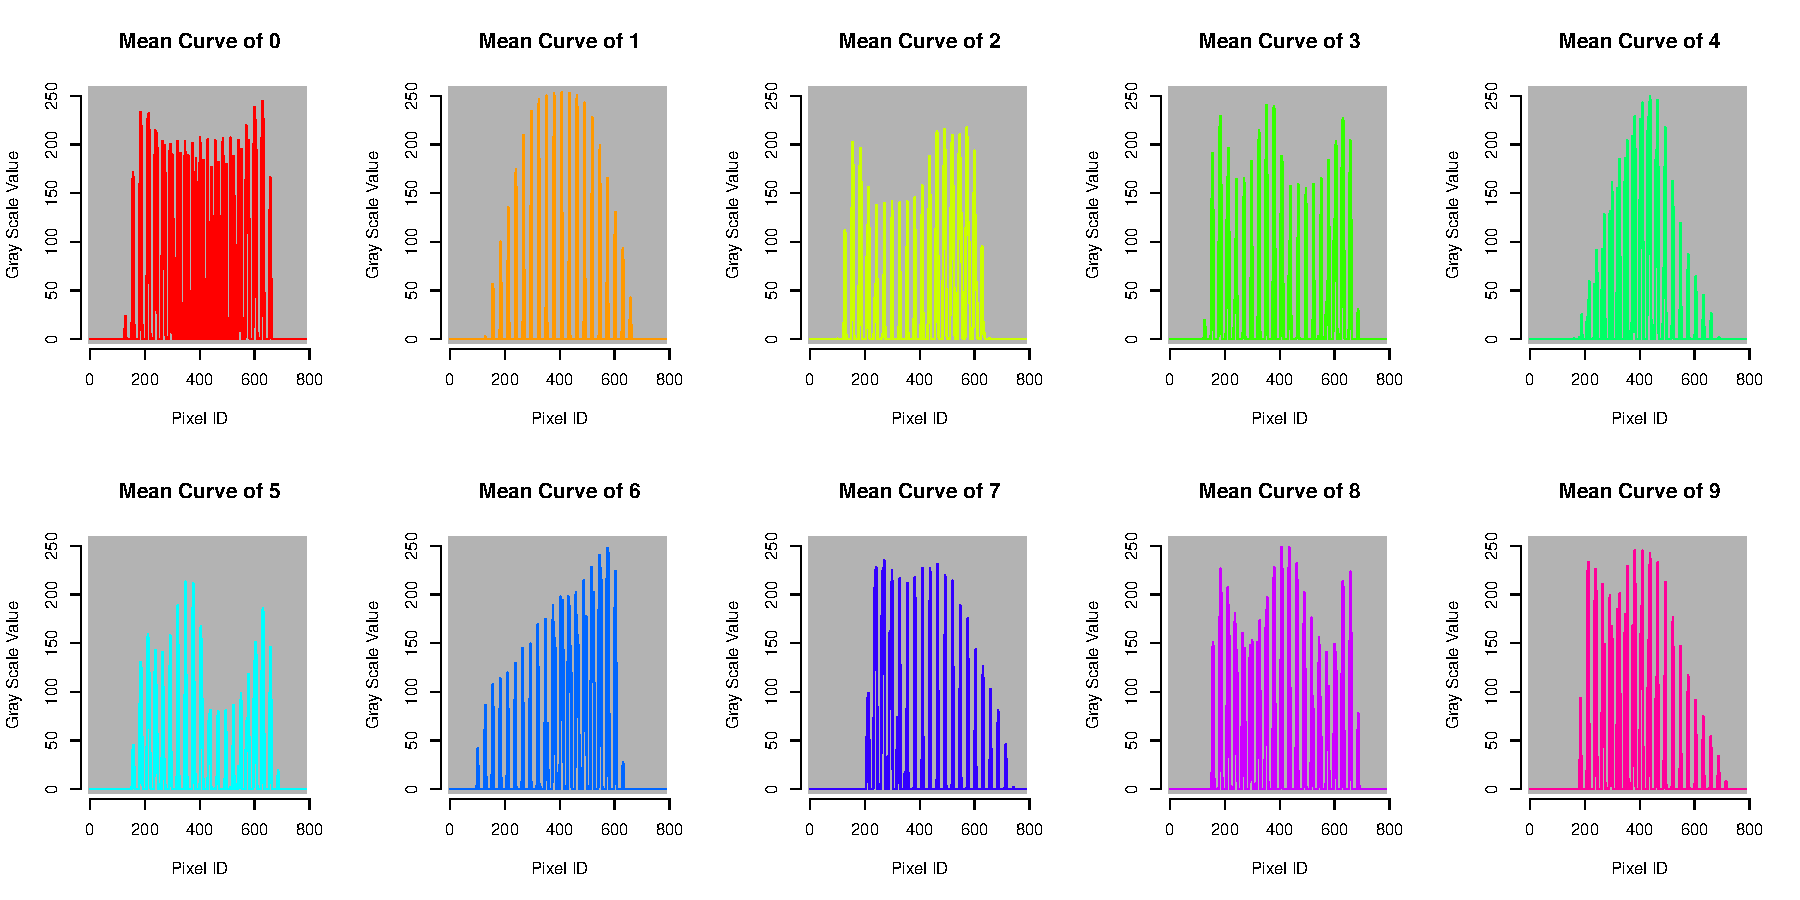
\includegraphics[width = 4.5 in]{figure/fig_mean_curve_trim.pdf}
\end{center}
\end{figure}
}

%%%%%%%%%%%%%%%%%%%%%%%%%%%%%%%%%%%%%%%%%%%%
%\subsection{Percentiles}
%\begin{frame}
%\frametitle{Change from the $1^{st}$ to the $99^{th}$ Percentiles}
%\begin{center}
%     \animategraphics[loop,controls,width=3.25 in]{12}{figure/fig_100tile_png/fig-}{0}{100}
%\end{center}
%\end{frame}

%%%%%%%%%%%%%%%%%%%%%%%%%%%%%%%%%%%%%%%%%%%%
\subsection{Principal Component Analysis}
\frame{
\frametitle{Coefficients for the Principal Component}
\begin{table}[htp]
\begin{center}
\begin{tabular}{c|cccccc}
			&	PC1		&	PC2   	&	$\cdots$	&	PC43	&	$\cdots$	&	PC784	\\ \hline
$pixel_0$		&	0.000 	&	\ 0.000  	&	$\cdots$	&	0.000	&	$\cdots$	&	\ 0.000	\\
$pixel_1$ 		&	0.000 	&	\ 0.000 	&	$\cdots$	&	0.000	&	$\cdots$	& \alert{-0.072}	\\
$\vdots$		&	$\vdots$	&	$\vdots$	&	$\ddots$	&	\vdots	&	$\ddots$	&	$\vdots$	\\
$pixel_{462}$ 	& \alert{0.075} 	&	-0.013 	&	$\cdots$ 	&	0.059  	&	$\cdots$	&	\ 0.000	\\
$\vdots$		&	$\vdots$	&	$\vdots$	&	$\ddots$	&	\vdots	&	$\ddots$	&	$\vdots$	\\
$pixel_{783}$	&	0.000 	&	\ 0.000  	&	$\cdots$ 	&	0.000	&	$\cdots$	&	\ 0.000	\\ \hline 
Variance		&	5.149 	&	\ 3.781  	&	$\cdots$	&	0.221	&	$\cdots$	&	\ 0.000	\\ \hline
Cumulative\\
Ratio of		&	0.098 	&	\ 0.169  	&	$\cdots$	&  \alert{0.800}	&	$\cdots$	&	\ 1.000	\\
Total Variance	&			&			&			&			&			&
\end{tabular}
\end{center}
\end{table}%
}

%%%%%%%%%%%%%%%%%%%%%%%%%%%%%%%%%%%%%%%%%%%%
\frame{
\frametitle{Cumulative Ratio of Total Variance}
\begin{figure}[htbp]
\begin{center}
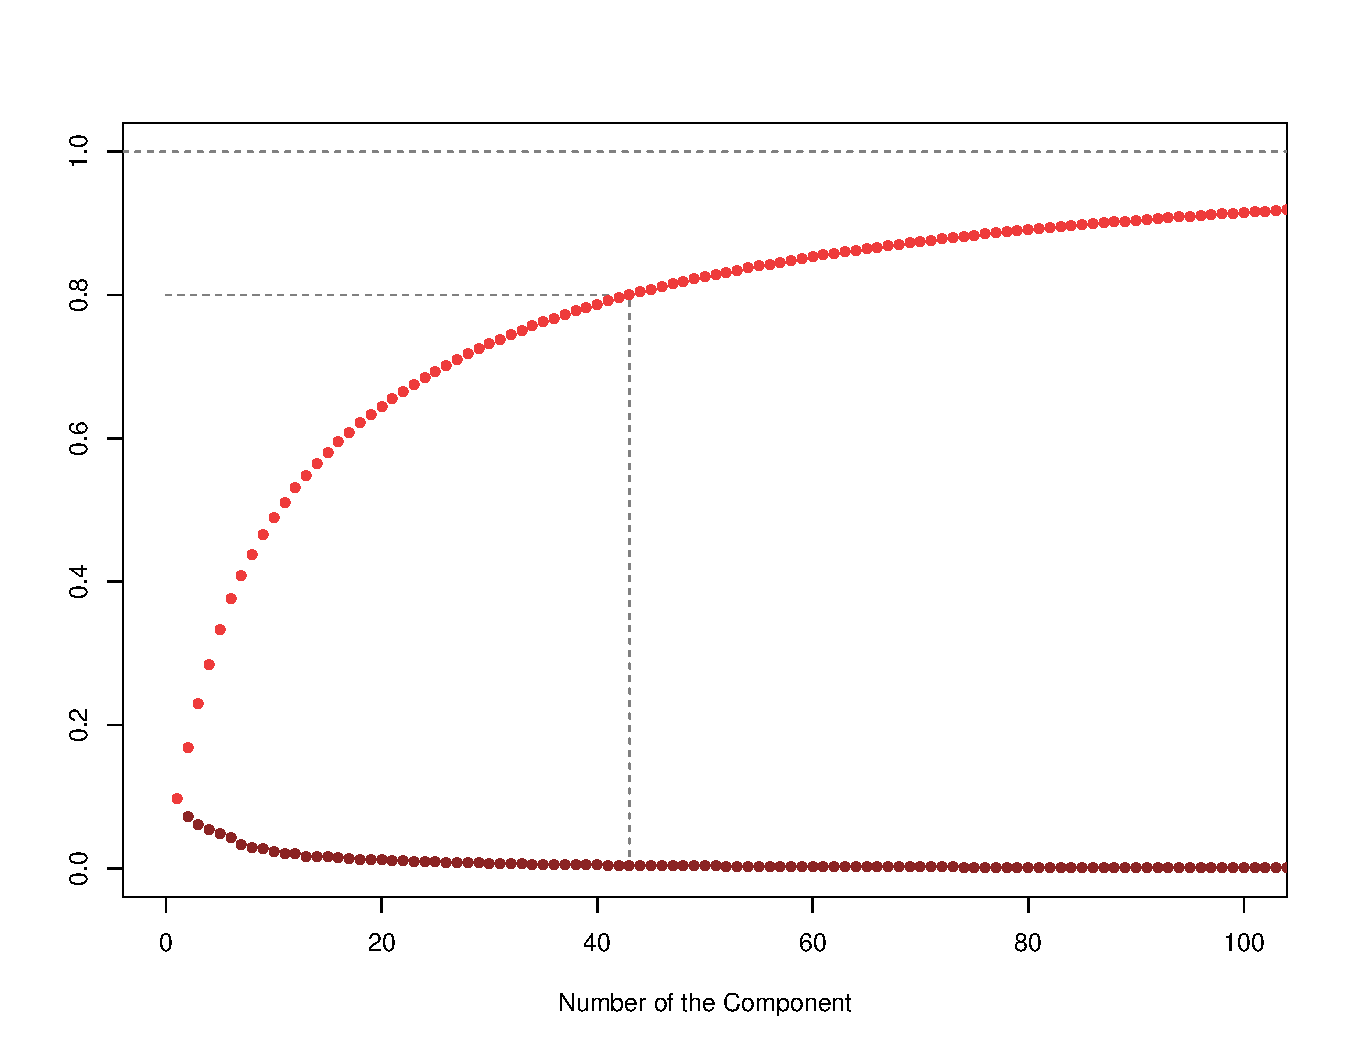
\includegraphics[width = 3.5 in]{figure/fig_pca_cum.pdf}
\end{center}
\end{figure}
}
%%%%%%%%%%%%%%%%%%%%%%%%%%%%%%%%%%%%%%%%%%%%
\frame{
\frametitle{Scatter Plot for the First Two Components}
\begin{figure}[htbp]
\begin{center}
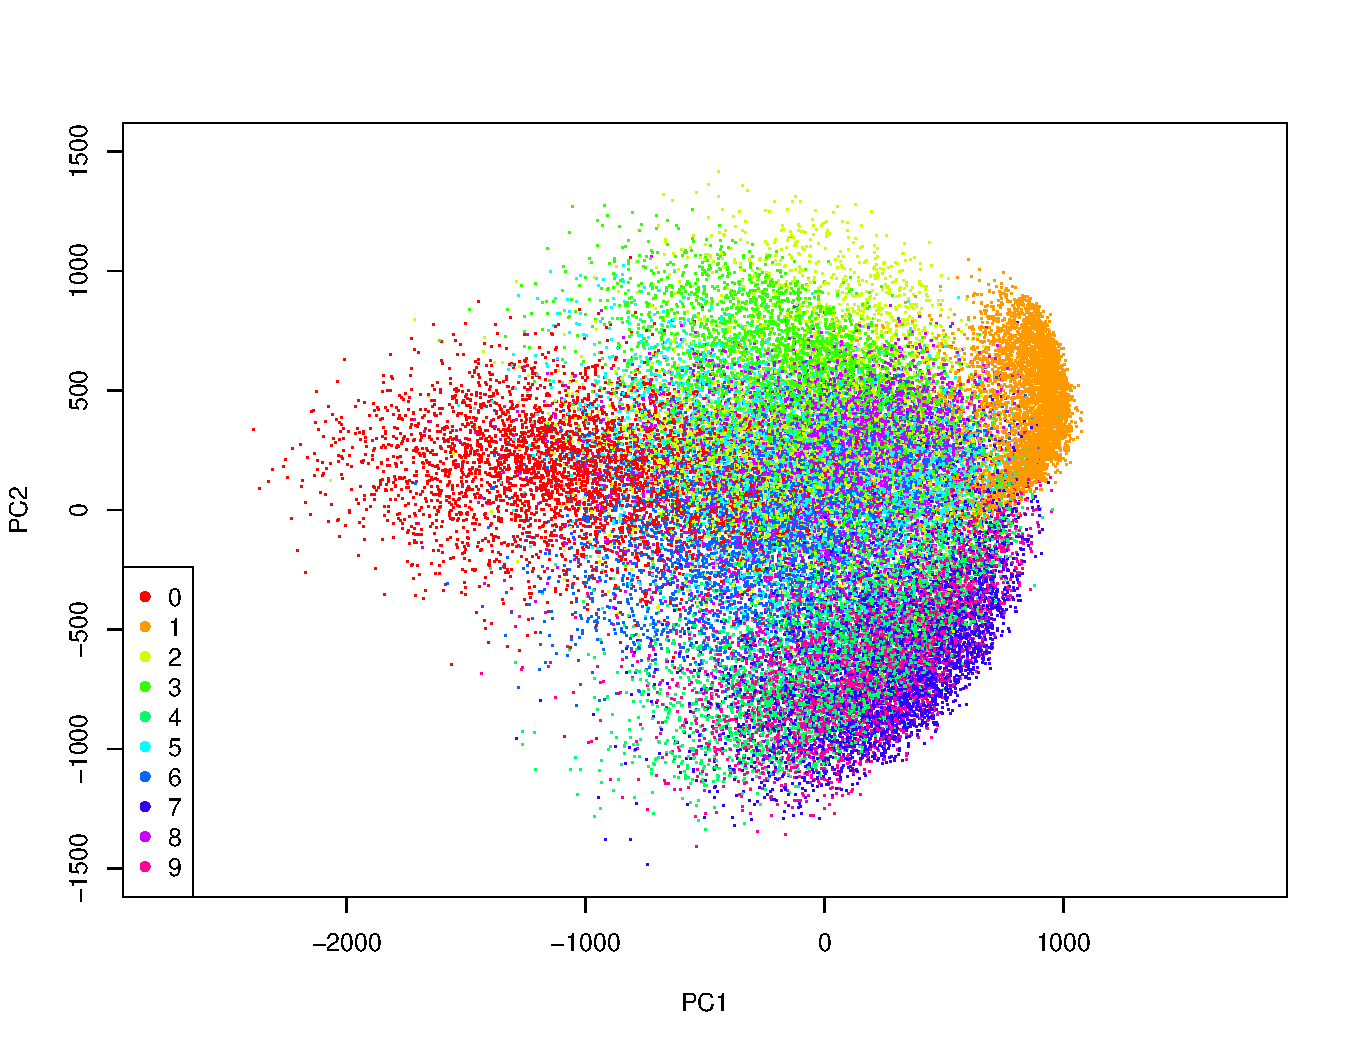
\includegraphics[width = 3.5 in]{figure/fig_pca_2.pdf}
\end{center}
\end{figure}
}

%%%%%%%%%%%%%%%%%%%%%%%%%%%%%%%%%%%%%%%%%%%%
\frame{
\frametitle{Separated Scatter Plot for the First Two Components}
\begin{figure}[htbp]
\begin{center}
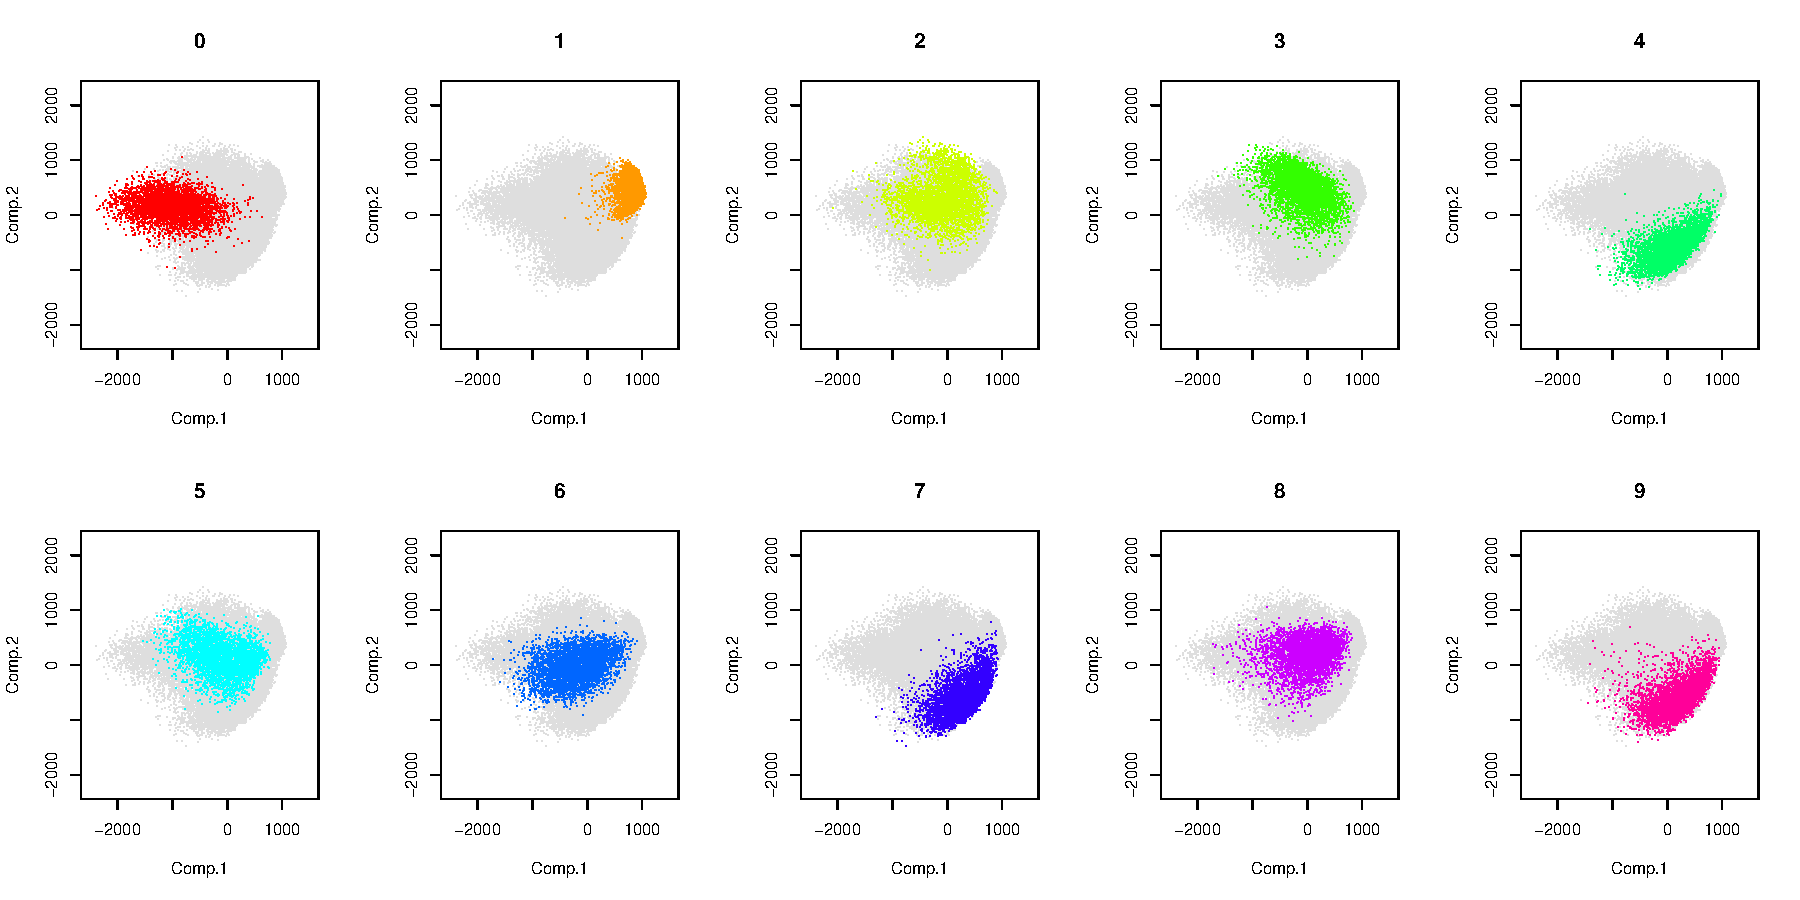
\includegraphics[width = 4.5 in]{figure/fig_pca_2_sep.pdf}
\end{center}
\end{figure}
}

%%%%%%%%%%%%%%%%%%%%%%%%%%%%%%%%%%%%%%%%%%%%
\subsection{t-SNE}
\frame{
\frametitle{Two-dimensional \href{http://distill.pub/2016/misread-tsne/}{t-SNE} with 600-time Iterations}
\begin{figure}[htbp]
\begin{center}
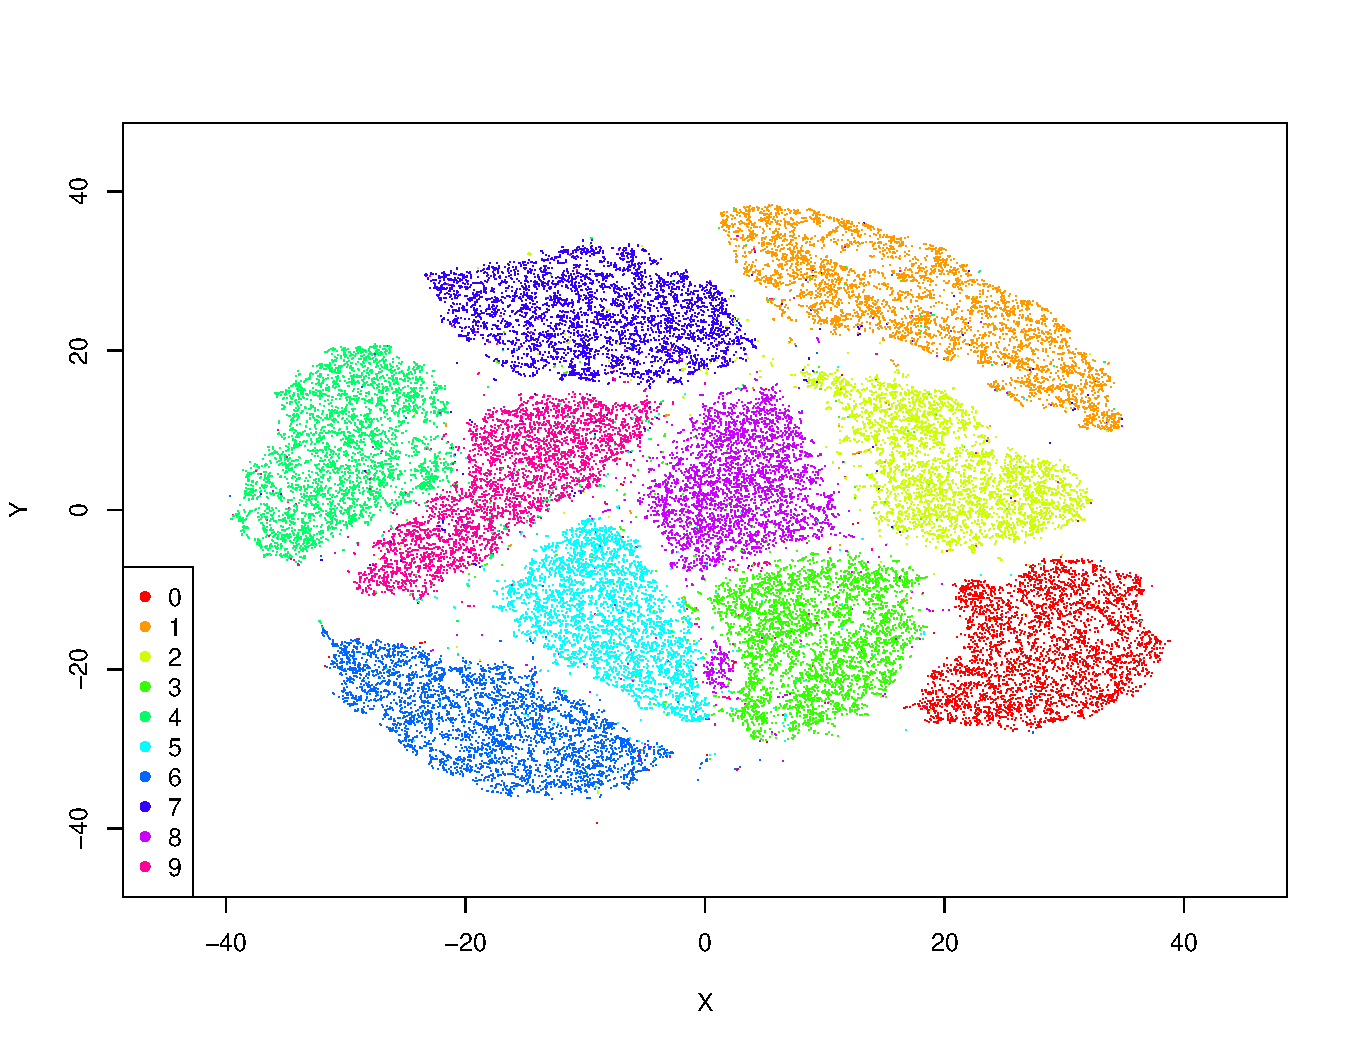
\includegraphics[width = 3.5 in]{figure/fig_tsne_2.pdf}
\end{center}
\end{figure}
\tiny

}

%%%%%%%%%%%%%%%%%%%%%%%%%%%%%%%%%%%%%%%%%%%%
\frame{
\frametitle{Separated Scatter Plot for the Two-dimensional t-SNE}
\begin{figure}[htbp]
\begin{center}
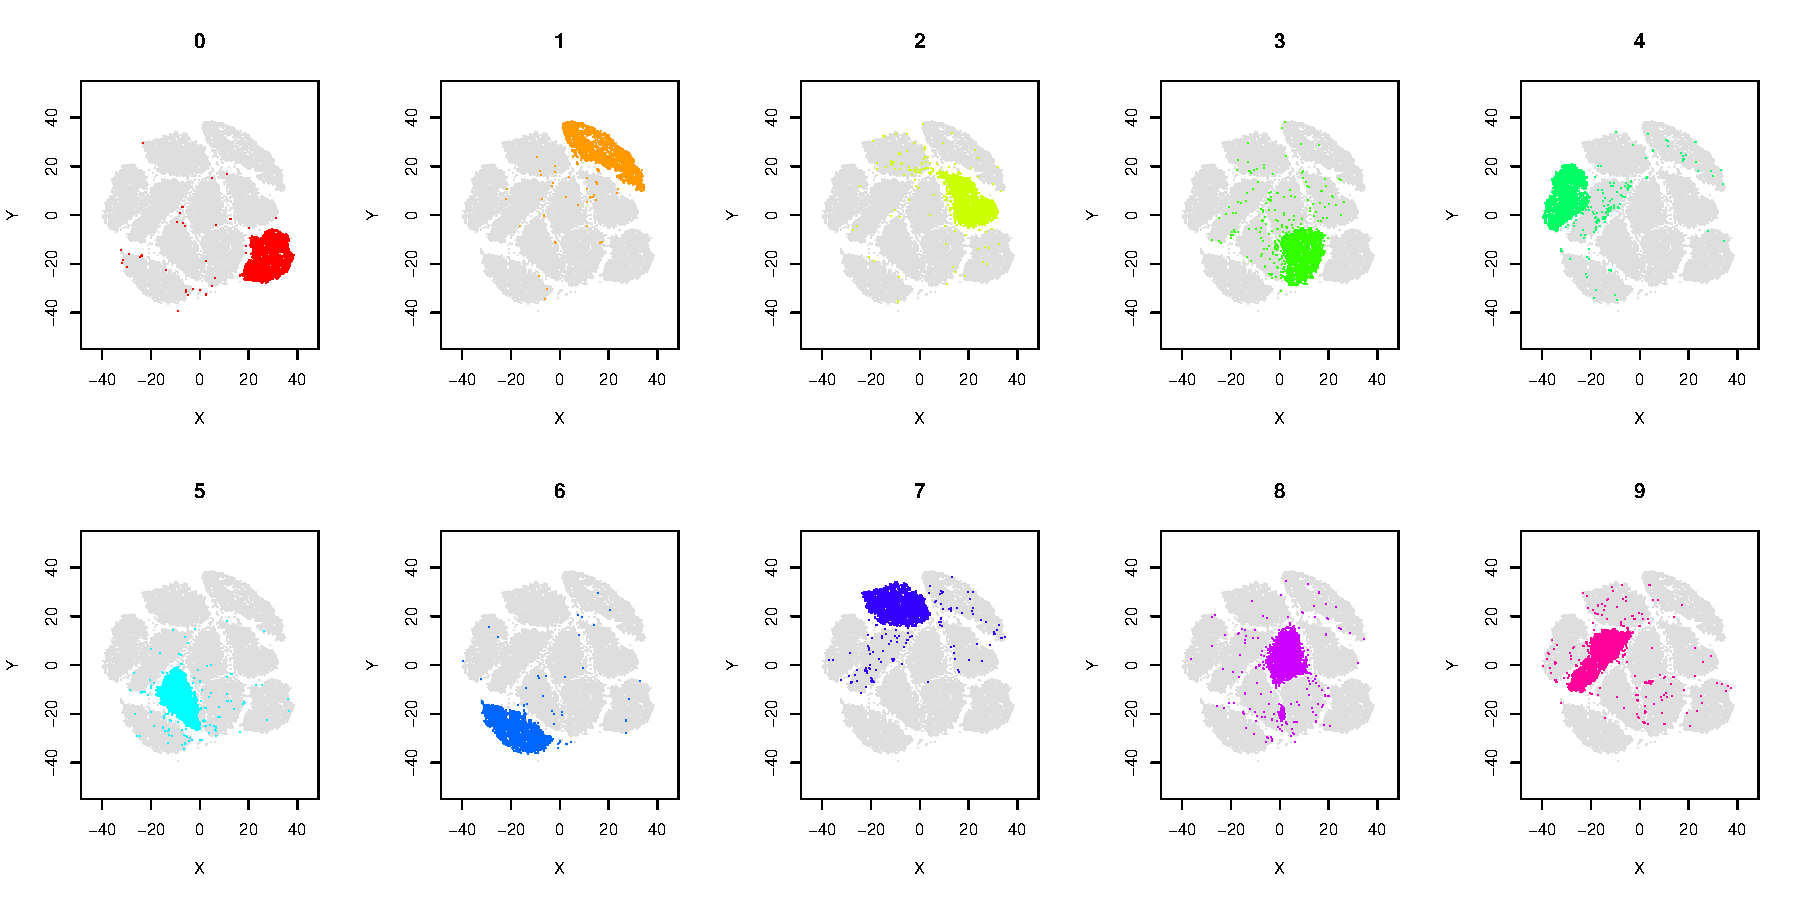
\includegraphics[width = 4.5 in]{figure/fig_tsne_2_sep.pdf}
\end{center}
\end{figure}
}

%%%%%%%%%%%%%%%%%%%%%%%%%%%%%%%%%%%%%%%%%%%%
\section{Analysis}
\subsection{Dimensionality Reduction}
\frame{
\frametitle{Dimensionality Reduction}
\begin{columns}

\begin{column}{.5\textwidth}
\begin{itemize}
\item Calculate the $90^{th}$ percentile
\item Preserve those pixels with non-zero $90^{th}$ percentile 
\item $43.75\%$ of pixels remain
\end{itemize}
\end{column}

\begin{column}{.5\textwidth}
\begin{figure}[htbp]
\begin{center}
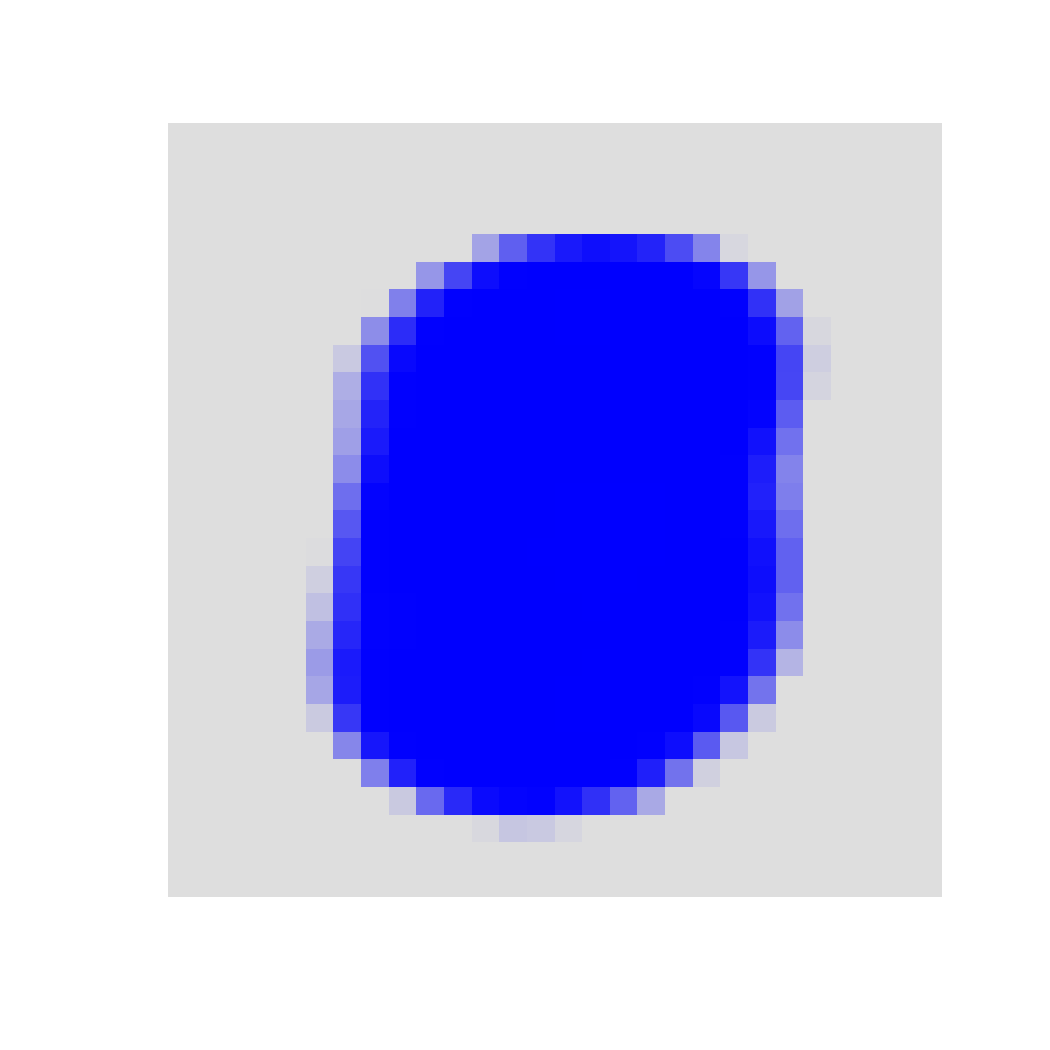
\includegraphics[width = \textwidth]{figure/fig_99tile.pdf}
\end{center}
\end{figure}
\end{column}

\end{columns}
}

%%%%%%%%%%%%%%%%%%%%%%%%%%%%%%%%%%%%%%%%%%%%
\subsection{One-versus-all Logistic Regression}
\frame{
\frametitle{One-versus-all Logistic Regression }
\begin{table}[htp]\footnotesize
\begin{center}
\begin{tabular}{c c | cccccccccc}
			&& \multicolumn{10}{c}{Prediction} \\
			&&	0	&	1	&	2   	&	3   	&	4   	&	5   	&	6   	&	7   	&	8   	&	9 \\ \hline
	\multirow{10}{*}{\begin{sideways}{Reality}\end{sideways}} 
  	&	0 	&	944  	&	7   	&	4   	&	9   	&	7   	&	1   	&	2   	&	1   	&	0   	&	0 \\
  	&	1 	&	536 	&	565  	&	8   	&	5   	&	4   	&	3   	&	4   	&	1   	&	2   	&	0 \\
  	&	2 	&	331 	&	291 	&	274 	&	13  	&	11  	&	10  	&	15  	&	10  	&	3   	&	1 \\
  	&	3 	&	251 	&	238 	&	244 	&	227  	&	20   	&	8   	&	8   	&	7   	&	2   	&	1 \\
  	&	4 	&	206 	&	173 	&	174 	&	196 	&	198  	&	14   	&	4   	&	5   	&	4   	&	5 \\
  	&	5 	&	154 	&	146 	&	166 	&	155 	&	141 	&	136  	&	10   	&	3   	&	4   	&	2 \\
  	&	6 	&	185 	&	135 	&	140 	&	116 	&	131 	&	142 	&	122  	&	0   	&	1   	&	0 \\
  	&	7 	&	148 	&	149 	&	131 	&	133 	&	141 	&	133 	&	127 	&	127  	&	5   	&	3 \\
  	&	8 	&	130 	&	120 	&	127 	&	105 	&	108 	&	109  &	78 	&	111  	&	77   	&	1 \\
  	&	9 	&	108 	&	117 	&	114 	&	114 	&	106  	&	96  	&	84 	&	100  	&	84  	&	78
\end{tabular}
\caption{Confusion Matrix (Accuracy $= 27.48\%$)}
\end{center}
\end{table}%
}

%%%%%%%%%%%%%%%%%%%%%%%%%%%%%%%%%%%%%%%%%%%%
\subsection{K-Nearest Neighbor}
\frame{
\frametitle{K-Nearest Neighbor (KNN)}
\begin{table}[htp]\footnotesize
\begin{center}
\begin{tabular}{c c | cccccccccc}
			&& \multicolumn{10}{c}{Prediction} \\
			&&	0	&	1	&	2   	&	3   	&	4   	&	5   	&	6   	&	7   	&	8   	&	9 \\ \hline
	\multirow{10}{*}{\begin{sideways}{Reality}\end{sideways}} 
	&	0  	&	963  	&	0    	&	2    	&	0    	&	2    	&	1    	&	3    	&	0    	&	0    	&	3	\\
  	&	1    	&	0 	&	1141	&	5    	&	1    	&	0    	&	1    	&	1    	&	1    	&	2    	&	0	\\
  	&	2    	&	6    	&	7  	&	979  	&	4    	&	1    	&	0    	&	1   	&	15    	&	1    	&	2	\\
  	&	3    	&	1    	&	0    	&	5  	&	957 	&	0   	&	17    	&	2   	&	6    	&	5    	&	3	\\
  	&	4    	&	0    	&	8    	&	0  	&	0  	&	957  	&	0    	&	6    	&	2    	&	0   	&	32	\\
  	&	5    	&	4    	&	1    	&	0   	&	18    	&	1  	&	827 	&	11    	&	3    	&	4    	&	4	\\
  	&	6    	&	5    	&	0    	&	1    	&	0    	&	3    	&	4  	&	957  	&	0    	&	0    	&	0	\\
  	&	7    	&	0    	&	8    	&	5    	&	0    	&	3    	&	0    	&	0 	&	1025	&	0    	&	7	\\
  	&	8    	&	3   	&	13    	&	5   	&	18    	&	3   	&	10    	&	5    	&	3  	&	885 	&	13	\\
  	&	9    	&	3    	&	3    	&	2   	&	6   	&	15    	&	2    	&	1   	&	19    	&	2  	&	955\end{tabular}
\caption{Confusion Matrix  (Accuracy $= 96.46\%$)}
\end{center}
\end{table}%
}


%%%%%%%%%%%%%%%%%%%%%%%%%%%%%%%%%%%%%%%%%%%%
\subsection{Support Vector Machine }
\frame{
\frametitle{Support Vector Machine (SVM)}
\begin{table}[htp]\footnotesize
\begin{center}
\begin{tabular}{c c | cccccccccc}
			&& \multicolumn{10}{c}{Prediction} \\
			&&	0	&	1	&	2   	&	3   	&	4   	&	5   	&	6   	&	7   	&	8   	&	9 \\ \hline
	\multirow{10}{*}{\begin{sideways}{Reality}\end{sideways}} 
	&	0  	&	961  	&	0    	&	5    	&	1    	&	0    	&	1	&	4    	&	0    	&	0    	&	2 	\\
  	&	1    	&	0 	&	1137	&	3    	&	3    	&	4    	&	1    	&	1    	&	2    	&	1    	&	0 	\\
  	&	2    	&	2    	&	1  	&	995  	&	1    	&	2    	&	1    	&	0    	&	5    	&	9    	&	0 	\\
  	&	3    	&	0    	&	0    	&	1  	&	974  	&	1    	&	7    	&	0    	&	3    	&	8    	&	2 	\\
  	&	4    	&	0    	&	3    	&	0    	&	0  	&	987  	&	0    	&	3    	&	0    	&	1   	&	11	\\
  	&	5    	&	1    	&	0    	&	0   	&	11    	&	1  	&	848 	&	6    	&	0    	&	3    	&	3	\\
  	&	6    	&	4    	&	0    	&	1    	&	0    	&	3    	&	4  	&	957  	&	0    	&	1    	&	0	\\
  	&	7    	&	0    	&	4    	&	3    	&	0    	&	1    	&	0    	&	0 	&	1034	&	1    	&	5	\\
  	&	8    	&	2    	&	2    	&	2    	&	2    	&	2    	&	4    	&	0    	&	1  	&	942  	&	1	\\
	&	9    	&	2    	&	2    	&	4    	&	6    	&	8    	&	1    	&	1    	&	4    	&	4  	&	976
\end{tabular}
\caption{Confusion Matrix  (Accuracy $= 98.11\%$)}
\end{center}
\end{table}%
}


%%%%%%%%%%%%%%%%%%%%%%%%%%%%%%%%%%%%%%%%%%%%
\subsection{Neural Network}
\frame{
\frametitle{Multi-layer Perceptron (784-1000-1000-10 with ReLU)}
\begin{table}[htp]\footnotesize
\begin{center}
\begin{tabular}{c c | cccccccccc}
			&& \multicolumn{10}{c}{Prediction} \\
			&&	0	&	1	&	2   	&	3   	&	4   	&	5   	&	6   	&	7   	&	8   	&	9 \\ \hline
	\multirow{10}{*}{\begin{sideways}{Reality}\end{sideways}} 
  	&	0	&	974	&	1	&	0	&	2	&	0	&	0	&	1	&	1	&	1	&	0 \\
	&	1	&	0	&	1128	&	2	&	0	&	0	&	0	&	3	&	0	&	2	&	0 \\
	&	2	&	1	&	1	&	1020	&	4	&	1	&	0	&	1	&	3	&	1	&	0 \\
	&	3	&	0	&	0	&	3	&	1000	&	0	&	2	&	0	&	3	&	0	&	2 \\
	&	4	&	1	&	0	&	2	&	1	&	966	&	0	&	4	&	1	&	1	&	6 \\
	&	5	&	2	&	0	&	0	&	11	&	1	&	873	&	4	&	0	&	0	&	1 \\
	&	6	&	2	&	3	&	0	&	1	&	3	&	5	&	944	&	0	&	0	&	0 \\
	&	7	&	0	&	6	&	11	&	2	&	0	&	1	&	0	&	1000 &	1	&	7 \\
	&	8	&	0	&	0	&	3	&	13	&	2	&	5	&	4	&	3	&	938	&	6 \\
	&	9	&	1	&	3	&	0	&	7	&	8	&	2	&	2	&	4	&	0	&	982 
\end{tabular}
\caption{Confusion Matrix  (Accuracy $= 98.25\%$)}
\end{center}
\end{table}%
}

%%%%%%%%%%%%%%%%%%%%%%%%%%%%%%%%%%%%%%%%%%%%

\frame{
\frametitle{Convolution Neural Network  }
\begin{table}[htp]\footnotesize
\begin{center}
\begin{tabular}{c c | cccccccccc}
			&& \multicolumn{10}{c}{Prediction} \\
			&&	0	&	1	&	2   	&	3   	&	4   	&	5   	&	6   	&	7   	&	8   	&	9 \\ \hline
	\multirow{10}{*}{\begin{sideways}{Reality}\end{sideways}} 
  	&	0	&	976	&	1	&	0	&	0	&	0	&	0	&	1	&	1	&	1	&	0 \\
	&	1	&	0	&	1134	&	0	&	1	&	0	&	0	&	0	&	0	&	0	&	0 \\
	&	2	&	1	&	2	&	1027	&	0	&	0	&	0	&	0	&	2	&	0	&	0 \\
	&	3	&	0	&	0	&	0	&	1005	&	0	&	3	&	0	&	0	&	2	&	0 \\
	&	4	&	0	&	0	&	0	&	0	&	980	&	0	&	0	&	0	&	0	&	2 \\
	&	5	&	0	&	0	&	0	&	5	&	0	&	886	&	1	&	0	&	0	&	0 \\
	&	6	&	1	&	3	&	0	&	0	&	2	&	4	&	946	&	0	&	2	&	0 \\
	&	7	&	0	&	3	&	5	&	1	&	0	&	0	&	0	&	1015	&	1	&	3 \\
	&	8	&	1	&	0	&	2	&	3	&	1	&	2	&	0	&	1	&	961	&	3 \\
	&	9	&	0	&	2	&	0	&	1	&	5	&	3	&	0	&	1	&	0	&	997
\end{tabular}
\caption{Confusion Matrix  (Accuracy $= 99.27\%$)}
\end{center}
\end{table}%
}

%%%%%%%%%%%%%%%%%%%%%%%%%%%%%%%%%%%%%%%%%%%%
\section{Predict Instantly Online}
\frame{
\frametitle{Predict Instantly Online}
\begin{itemize}
\item \url{https://goo.gl/Ac1aXg}
\item Train the MLP with Keras on Python
\item Export the weight matrices and bias vectors as JavaScript file
\item Insert the matrices into JavaScript
\item \alert{Mobilized} the model
\end{itemize}
}
%%%%%%%%%%%%%%%%%%%%%%%%%%%%%%%%%%%%%%%%%%%%
\frame{
\center{Q \& A}
}

\frame{
\center{Thank you for listening}
}

\end{document}
